% Options for packages loaded elsewhere
\PassOptionsToPackage{unicode}{hyperref}
\PassOptionsToPackage{hyphens}{url}
%
\documentclass[
  12pt,
]{article}
\usepackage{lmodern}
\usepackage{amsmath}
\usepackage{ifxetex,ifluatex}
\ifnum 0\ifxetex 1\fi\ifluatex 1\fi=0 % if pdftex
  \usepackage[T1]{fontenc}
  \usepackage[utf8]{inputenc}
  \usepackage{textcomp} % provide euro and other symbols
  \usepackage{amssymb}
\else % if luatex or xetex
  \usepackage{unicode-math}
  \defaultfontfeatures{Scale=MatchLowercase}
  \defaultfontfeatures[\rmfamily]{Ligatures=TeX,Scale=1}
  \setmainfont[]{Times New Roman}
\fi
% Use upquote if available, for straight quotes in verbatim environments
\IfFileExists{upquote.sty}{\usepackage{upquote}}{}
\IfFileExists{microtype.sty}{% use microtype if available
  \usepackage[]{microtype}
  \UseMicrotypeSet[protrusion]{basicmath} % disable protrusion for tt fonts
}{}
\makeatletter
\@ifundefined{KOMAClassName}{% if non-KOMA class
  \IfFileExists{parskip.sty}{%
    \usepackage{parskip}
  }{% else
    \setlength{\parindent}{0pt}
    \setlength{\parskip}{6pt plus 2pt minus 1pt}}
}{% if KOMA class
  \KOMAoptions{parskip=half}}
\makeatother
\usepackage{xcolor}
\IfFileExists{xurl.sty}{\usepackage{xurl}}{} % add URL line breaks if available
\IfFileExists{bookmark.sty}{\usepackage{bookmark}}{\usepackage{hyperref}}
\hypersetup{
  pdftitle={Methane Emissions Status for Manure Management across USA},
  pdfauthor={Nadia Swit and Kendra Sultzer},
  hidelinks,
  pdfcreator={LaTeX via pandoc}}
\urlstyle{same} % disable monospaced font for URLs
\usepackage[margin=2.54cm]{geometry}
\usepackage{graphicx}
\makeatletter
\def\maxwidth{\ifdim\Gin@nat@width>\linewidth\linewidth\else\Gin@nat@width\fi}
\def\maxheight{\ifdim\Gin@nat@height>\textheight\textheight\else\Gin@nat@height\fi}
\makeatother
% Scale images if necessary, so that they will not overflow the page
% margins by default, and it is still possible to overwrite the defaults
% using explicit options in \includegraphics[width, height, ...]{}
\setkeys{Gin}{width=\maxwidth,height=\maxheight,keepaspectratio}
% Set default figure placement to htbp
\makeatletter
\def\fps@figure{htbp}
\makeatother
\setlength{\emergencystretch}{3em} % prevent overfull lines
\providecommand{\tightlist}{%
  \setlength{\itemsep}{0pt}\setlength{\parskip}{0pt}}
\setcounter{secnumdepth}{5}
\ifluatex
  \usepackage{selnolig}  % disable illegal ligatures
\fi

\title{Methane Emissions Status for Manure Management across USA}
\usepackage{etoolbox}
\makeatletter
\providecommand{\subtitle}[1]{% add subtitle to \maketitle
  \apptocmd{\@title}{\par {\large #1 \par}}{}{}
}
\makeatother
\subtitle{\url{https://github.com/sultzerk/SultzerSwit_ENV872_EDA_FinalProject.git}}
\author{Nadia Swit and Kendra Sultzer}
\date{}

\begin{document}
\maketitle

\newpage
\tableofcontents 
\newpage
\listoftables 
\newpage
\listoffigures 
\newpage

\hypertarget{rationale-and-research-questions}{%
\section{Rationale and Research
Questions}\label{rationale-and-research-questions}}

For this project, we were interested in manure management and greenhouse
gas emissions created by livestock. Our initial dataset considered
methane, nitrous oxide, and carbon dioxide. Research revealed that
``livestock are reckoned to be responsible for up to 14\% of all
greenhouse emissions from human activities'' (BBC article). With such a
substantial amount of human activities, we wanted to see how livestock
factored into emissions. When considering different emissions types, we
focused on methane because methane is a very detrimental greenhouse gas:
it traps heat at a rate 25 times greater than carbon dioxide (BBC
article). Methane gas explored here is produced by the anaerobic
decomposition of manure stored or treated.

Question:

\emph{\emph{Question 1: Have methane emissions changed over time?}}

\begin{itemize}
\tightlist
\item
  Create time series of methane produced by one or two livestock for
  general trend
\item
  Use CH4 emissions variable -- want to see if the gigagrams of methane
  have increased over time
\item
  Filter for one element for time series?
\end{itemize}

\_* Question 2: Does the average methane emissions rate differ between
each animal category?*\_ Specifically:

\begin{itemize}
\tightlist
\item
  Is there a difference in rate produced by each animal? Looking for
  statistical difference between the rates of different livestock
\item
  Run an ANOVA test - check whether or not there is a significant
  difference between livestock
\item
  Use the Implied emissions factor variable
\item
  Make fancy summary tables
\end{itemize}

\newpage

\hypertarget{dataset-information}{%
\section{Dataset Information}\label{dataset-information}}

Dataset used for this project was found from the Food \& Agriculture
Organization of the United Nations (FAO), specifically from FAOSTAT.
FAOSTAT provides free access to statistics pertaining to agriculture and
for over 245 countries. For this analysis, we focused on emissions in
the United States. \emph{more info on how data was collected}

Metadata!

\textbf{what values should be in the table? total dataset or just
specific to methane and our years? }Remember to create README file
**remmber to write csv's for all processed data

\newpage

\hypertarget{exploratory-analysis}{%
\section{Exploratory Analysis}\label{exploratory-analysis}}

\hypertarget{data-wrangling-steps}{%
\subsection{Data wrangling steps}\label{data-wrangling-steps}}

First, we viewed a summary of our data to decide how to pare it down and
wrangle it.

We wanted to make our dataset more manageable, so we filtered for the
specific columns we wanted to retain, the variable we were interested in
(methane emissions), and only focused on the past years.

\hypertarget{basic-visualizations}{%
\subsection{Basic visualizations}\label{basic-visualizations}}

First, when considering our first research question, we wanted to see
how methane emissions appear over time. When combining all animals, we
can see there is a general increasing trend over time (Figure 1).
However, there is a sharp decrease in methane emissions at the beginning
of the dataset (\textasciitilde1980-1985) that might warrent
investigation later. For our analysis, we wanted to investigate whether
this trend was significant.

\begin{figure}
\centering
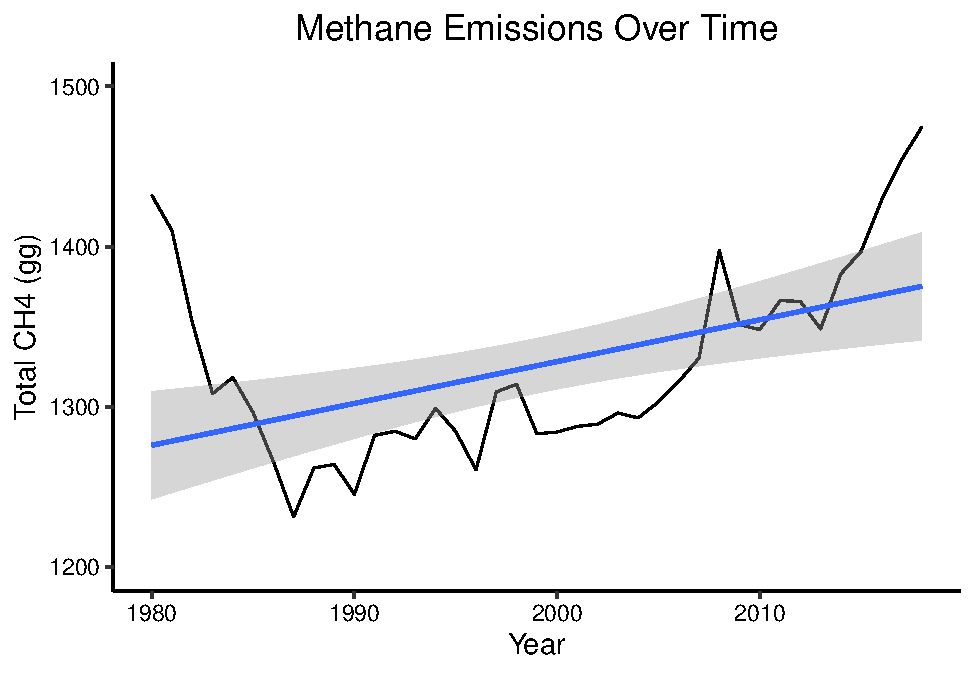
\includegraphics{Methane_Project_Template_files/figure-latex/unnamed-chunk-2-1.pdf}
\caption{Methane Emissions Over Time}
\end{figure}

Our second research question focused on the different emission rates
between animals. We were curious about this question when we explored a
boxplot showing the different rates (Figure 2). According to this
boxplot, we suspected that there might be statistical differences since
for, example: dairy cattle and market swine had higher rates than
others.

\begin{figure}
\centering
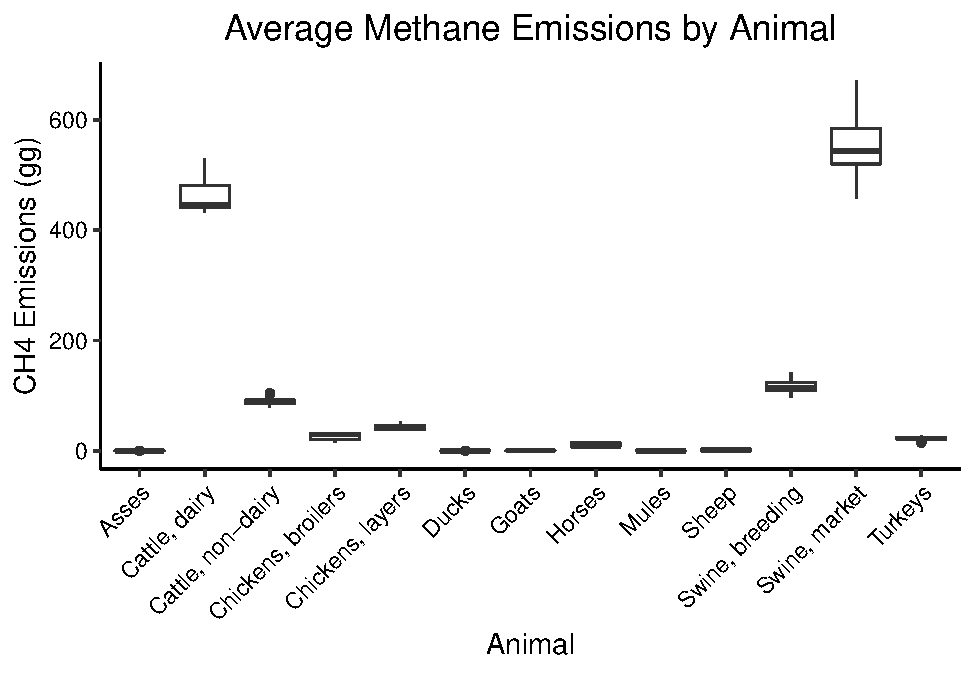
\includegraphics{Methane_Project_Template_files/figure-latex/viewing boxplot of methane by animal-1.pdf}
\caption{Average Methane Emissions by Animal}
\end{figure}

\newpage

\hypertarget{analysis}{%
\section{Analysis}\label{analysis}}

\hypertarget{research-question-1}{%
\subsection{Research Question 1}\label{research-question-1}}

To answer our first research question, we conducted a time series on the
overall methane production for all livestock. Since methane was only
calculated once a year, there was no seasonality to our data, and we
were not able to decompose our time series. However, we conducted a
Mann-Kendall test, which confirmed that there was a significant trend
(p-value \textless{} 0.05). From our data exploration, we can say that
overall that trend is increasing: methane emissions between 1980 and
2018 have increased across 13 livestock in the United States.

\hypertarget{research-question-2}{%
\subsection{Research Question 2}\label{research-question-2}}

To answer the second research question, we conducted a one-way ANOVA
test to evaluate whether the different animals, on average, have
different emission rates. To begin this process, we had to test the
emission rates for normality. The important assumption for generalized
linear models is the normality of residuals. The Shapiro-Wilk test
showed that, of the 13 livestock, only ducks, breeding swine, and market
swine were normally distributed. When viewing a Q-Q plot, once can see
the data does not follow a normal distribution (Figure 3). Lastly,
Bartlett's test for homogeneity of variances was run, which revealed
that the variances were not equal (p \textless{} 0.05). Even though all
of the tests for normality failed, we proceeded on with the analysis.

\begin{figure}
\centering
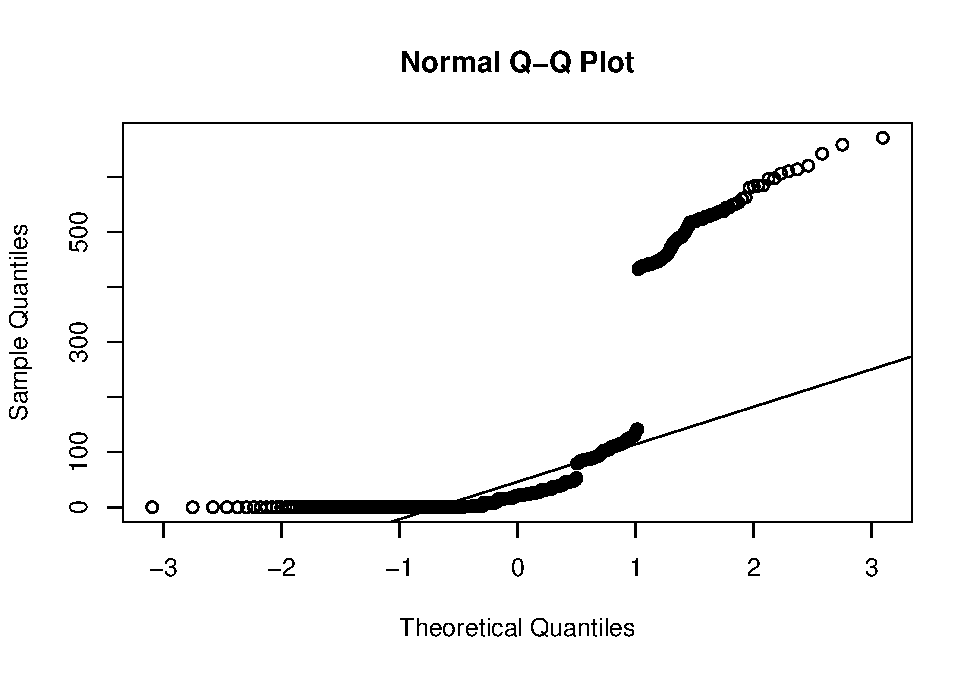
\includegraphics{Methane_Project_Template_files/figure-latex/unnamed-chunk-4-1.pdf}
\caption{QQ plot}
\end{figure}

Our analysis then revealed that there was a significant difference in
mean emissions among animals (ANOVA; F: 4394 on 12 and 494
DF,p\textless0.05). But which animals had different means? A Tukey's HSD
test helped show which means were different between the animals. We
extracted groupings for pair-wise relationships where the letters in
Figure 4 represent the different groupings. Thus, asses, ducks, goats,
mules, and sheep all had statistically similar emission rates (Figure
4). Most of the other animals, such as market swine and dairy cattle,
have their own grouping.

\begin{figure}
\centering
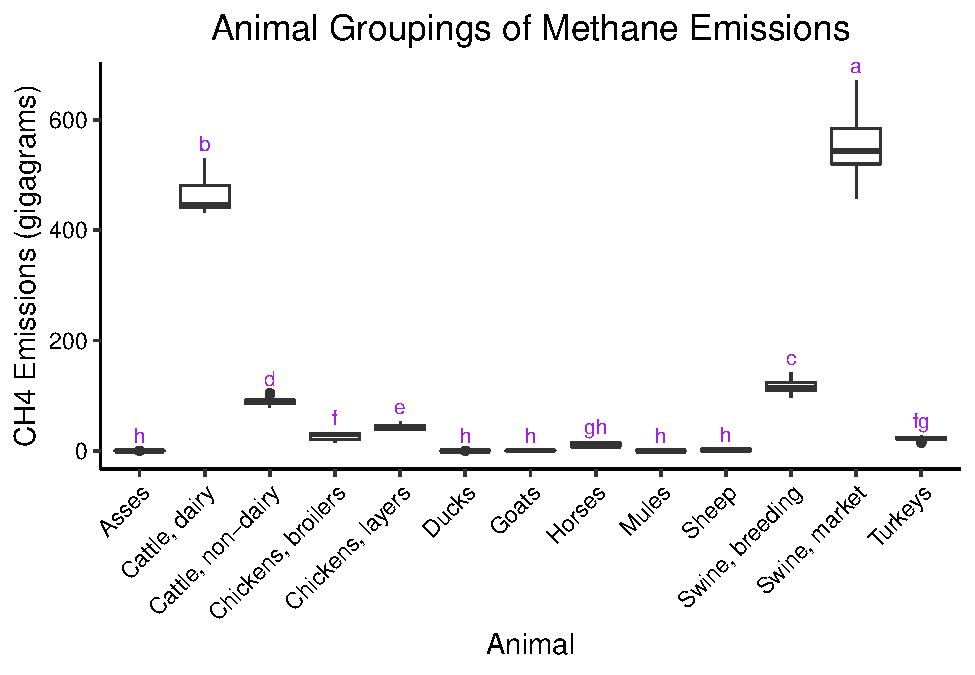
\includegraphics{Methane_Project_Template_files/figure-latex/anova results-1.pdf}
\caption{Animal Groupings of Methane Emissions}
\end{figure}

Nadia: Time series Kendra: ANOVA and grouping

\newpage

\hypertarget{summary-and-conclusions}{%
\section{Summary and Conclusions}\label{summary-and-conclusions}}

Conclusions from time series and ANOVA Include normality test results

\newpage

\hypertarget{references}{%
\section{References}\label{references}}

BBC citation article:
\url{https://www.bbc.com/future/article/20190806-how-vaccines-could-fix-our-problem-with-cow-emissions}
\textless add references here if relevant, otherwise delete this
section\textgreater{}

\end{document}
